\label{app:A}

Simulamos a resposta de frequência de uma sala utilizando o algoritmo Image-Source Model \cite{simulation}.

sala utilizada nas simulações tem dimensões 4,45m × 3, 55m × 2,5m (largura × comprimento × altura). A sala é completamente selada, para fins de simulação. Além disso, o coeficiente de absorção de todos os lados é o mesmo, como se todos fossem feitos do mesmo material. O material utilizado varia com o tempo de reverberação, e o algoritmo de simulação calcula o coeficiente de absorção de cada lado da sala dependendo do
tempo de reverberação escolhido. O arranjo de microfones é linear e foi montado em torno do ponto $\mathpzc{Mic_c = [2 1,5 1,6]^T}$. São 2 microfones e fontes. As fontes foram distribuídas em torno do centro do arranjo, com dois parâmetros para identificá-las: o DOA de cada uma, e a distância delas até o arranjo. O parâmetro mais importante da sala é o tempo de reverberação. O tempo utilizado nesta dissertação é o $\mathpzc{T_60}$, que é o tempo requerido para que as reflexões cheguem a 60 dB abaixo do nível do som direto.

As fontes utilizadas foram do SASSEC e são trechos de sinal de voz de 10 segundos de duração cada, amostrados a 16 kHz. Decimamos os sinais para que a frequência de amostragem caísse para 8 kHz. As projeções do ambiente estão representados na Figura \ref{fig:environment}

\begin{figure}
    \centering
    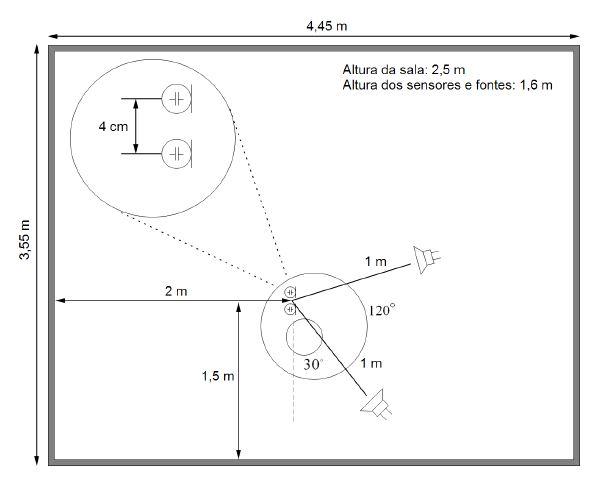
\includegraphics{environment.JPG}
    \caption{Configuração da sala utilizada nos testes.}
    \label{fig:environment}
\end{figure}